\documentclass[aspectratio=169, 10pt, handout,usenames,dvipsnames]{beamer}

\usecolortheme{dove}
\definecolor{mycyan}{rgb}{0.2157, 0.7059, 0.9608}
\setbeamercolor{alerted text}{fg=mycyan}
\setbeamertemplate{bibliography item}{\insertbiblabel}
\setbeamertemplate{caption}[numbered]
\hypersetup{colorlinks,linkcolor=,urlcolor=mycyan}
\usepackage{animate,xcolor,colortbl,listings,nicefrac}
\usepackage[italian]{babel}
\usepackage{verbatim}
\usepackage{mathtools}
\setbeamertemplate{footline}[frame number]
\usepackage{listings}
\lstset{upquote=false}
\usepackage[]{framed}
\usepackage{xfrac}
\usepackage{multicol}
\usepackage{cellspace}
\usepackage{tikz}
\usepackage[american,europeanvoltages]{circuitikz}
\setlength\cellspacetoplimit{4pt}
\setlength\cellspacebottomlimit{4pt}
\setbeamercolor{alerted text}{fg=Cerulean}

\newcommand{\circuito}{    
    \draw (0,0) 
        to[sV, l=$V_{in}$] (0,3) 
        -- (0.5,3)
        to[L=$L$] (2,3) 
        to[R=$R1$] (5,3)
        to[R=$R2$] (5,0)
        -- (0,0);
    \draw (5,3) 
        -- (7,3) 
        to[C, l=$C$] (7,0) -- (5,0);
    \draw 
        (7,3) to[short, -o]
        node[anchor=west]{} (8,3);
    \draw 
        (7,0) to[short, -o]
        node[anchor=west]{} (8,0);
    \draw 
     (8,3) to[open, v^<=$V_{out}$] (8,0); }
\begin{document}


\begin{frame}
  \title{Metodi multistep: BDF e sistemi stiff}
  
  \date{27/05/2020}
  \author{Giacomo Tombolan \and Valerio Nappi \and 
          Lorenzo Rossi \and  \\Marco Manganini \and
          Mirko Seghezzi}
  \maketitle
\end{frame}


\begin{frame}


  \frametitle{Bibliografia}
  \begin{thebibliography}{99}\small
    
    \bibitem{quarteroni2012calcolo}
    Quarteroni A., Saleri F. and Gervasio P.
    \newblock {\em Calcolo Scientifico: Esercizi e problemi risolti con MATLAB e  Octave}.
    \newblock UNITEXT. Springer Milan, 2012.

    \bibitem{petzold}
    Ascher Uri M. and Petzold Linda R.
    \newblock {\em Computer methods for ordinary differential equations and differential-algebraic equations}.
    \newblock Siam, 1998.

    \bibitem{robertson}
    Robertson H. H. "The Solution of a Set of Reaction Rate Equations"
    \newblock {in: Walsh J. (ed.), \em Numerical Analysis. An Introduction based on a Symposium Organized by the Institute of Mathematics and its Applications}.
    \newblock Academic Press, 1972. pp 178-182
  

   \end{thebibliography}

%Una volta inserito un documento in bibliografia, 
%può essere citato così:~\cite{quarteroni2012calcolo}
  
\end{frame}  




\begin{frame}
  \frametitle{Sommario}
  %Questo comando inserisce una lista delle sezioni in
  %cui è divisa la presentazione. Perché una sezione appaia 
  %nel sommario deve contenere almeno una pagina.
  \tableofcontents
\end{frame}




\begin{comment}
        \begin{frame} \frametitle{Come inserire una formula}

        Una formula può essere inserita all'interno del testo così : 
        $-\nabla \left( \varepsilon \nabla u \right) = f $ oppure 
        centrata e numerata così:
        \begin{equation}\label{eq:poisson}
            -\nabla \cdot \left( \varepsilon \nabla u \right) = f
        \end{equation}
        oppure centrata senza numerazione così :
        $$
         -\nabla \cdot \left( \varepsilon \nabla u \right) = f
        $$
        Posso fare riferimento alle formule numerate così : \eqref{eq:poisson}
        \end{frame}
        
        \begin{frame} \frametitle{Come inserire una lista per punti}
        Ecco come inserire una lista per puti
        \begin{itemize}
            \item un punto
            \item un altro
        \end{itemize}
        oppure un elenco numerato
        \begin{enumerate}
            \item primo punto
            \item secondo punto
        \end{enumerate}

        \end{frame}
        
        
        \begin{frame} \frametitle{Come inserire un pezzo di codice}
        Si può evidenziare \alert{parte del testo} in questo modo.
        %
        Si può inserire un comando matlab all'interno del testo
        in questo modo : \lstinline[language=Matlab]{for i = 1 : 10, disp (i), end}
        
        si può inserire un un file contenete un codice matlab in questo modo :
        \lstinputlisting[language=Matlab]{codice.m}
        
        Si possono inserire solo alcune righe del file in questo modo :
        \lstinputlisting[language=Matlab, firstline=1, lastline=2]{codice.m}
        
        \end{frame}


\end{comment}

\section{Introduzione a sistemi stiff e metodi BDF}\label{sec:sec1}
\begin{frame} \frametitle{Introduzione a sistemi stiff e metodi BDF}
    \begin{itemize}
        \item I sistemi stiff sono problemi molto comuni nel campo dell'elettronica. 
        \item Analizzeremo dei metodi per risolverli efficacemente
        \item Ma prima di dare definizioni...
    \end{itemize}
\end{frame}

    
\begin{comment}
%COMMENTATO LA SEZIONE REAZIONE CHIMICA DI ROBERTSON E APPLICAZIONI DEI SISTEMI STIFF

\section{Applicazioni}\label{sec:sec2}
    \begin{frame}{Applicazioni}
            \begin{itemize}
                \item Automatica: progettazione di controllori il più reattivi possibile alle perturbazioni 
                \item Elettronica: simulazione circuitale.\\
                \medskip 
                \medskip
                N.B.: i nodi formati da componenti senza memoria (diodi, resistenze, etc) formano le Differential Algebraic Equations (DAEs) : autovalori caratterizzanti del sistema a velocità infinita
    
            \end{itemize}       
    \end{frame}



\section{Sistemi stiff: una reazione chimica}
\begin{frame}{Esempio: una reazione chimica stiff - la reazione di Robertson}
\begin{itemize}
    \item Il problema ROBER descrive la cinetica di una reazione autocatalitica la cui struttura può essere rappresentata come: \newline
    \begin{center}
        \begin{cases} 
            A \xrightarrow{k_1} B \\
            B + B \xrightarrow{k_2} C + B \\
            B + C \xrightarrow{k_3} A + C
        \end{cases} 
    \end{center}
    \newline
    dove $A$, $B$ e $C$ sono le specie chimiche coinvolte e $k_1$, $k_2$ e $k_3$ sono le costanti di velocità, che assumono valori molto diversi ( $k_1 = 0.04$, $k_2=3\cdot10^7$ e $k_3=10^4$)
    \item La grande differenza tra costanti di velocità dà origine ad un sistema stiff. Infatti, questo tipo di reazione ha una velocità iniziale molto alta per poi evolversi molto lentamente nel tempo.
    \item Mentre nella seconda parte basterebbe un passo $ h $ molto piccolo, nella prima parte ciò non sarebbe sufficiente
\end{itemize}
\end{frame}
\end{comment}
    
\section{Sistemi stiff: circuito RLC}\label{sec:sec3}

\begin{frame}{Circuito RLC}
Si supponga di prendere in esame il seguente circuito, con l'obiettivo di calcolarne la tensione di uscita \( V_{out} \) considerando un generatore di tensione forzante \( V_{in} \)

            \begin{center}
                    \begin{circuitikz}[scale=1]
                \circuito
                \end{circuitikz}
            \end{center}

\end{frame}

\begin{frame}{Analisi del circuito RLC}
Analizziamo il circuito attraverso la legge di Kirchhoff delle correnti e quella delle tensioni. Prendiamo in considerazione la maglia \textcolor{Cerulean}{azzurra} e il nodo \textcolor{BurntOrange}{arancione}.
\vspace{0.3cm}
    \begin{multicols}{2}
    \begin{center}
    \hspace*{-0.5cm}
        \begin{circuitikz}[scale=0.8]
        \circuito
        \draw [Cerulean, thick, latex-] (2.5,0.5) arc (-90:175:10mm) ;
        \draw [Cerulean] (2.5,1.5)node{KLV}
        \draw [BurntOrange, thick] (4.5,3.6) rectangle (7.5,2.6)
        \draw [BurntOrange] (6,3) node[above] {KLC};
        \end{circuitikz}
    \end{center}
    
    \columnbreak
    
    \hspace*{1.7cm}\begin{minipage}{\textwidth}
        \large
        \begin{cases}
           \textcolor{Cerulean}{KLV:} V_{in} = V_L + V_{R1} + V_{out}  \\
           \textcolor{BurntOrange}{KLC:} I_{L} =  I_{R2} + I_C\;
        \end{cases} 
        \medskip\\
        \begin{cases}
            {x_1} = V_{out}\\
            {x_2} = I_L \;
        \end{cases} 
        \bigskip\\
        Otteniamo il sistema:\medskip\\
        \begin{cases}
            \dot{x_1} = -\dfrac{1}{L}x_1 - \dfrac{R1}{L}x_2 + \dfrac{1}{L}V_{in}\\
            \dot{x_2} = -\dfrac{1}{R2C}x_1 + \dfrac{1}{C}x_2  \;
        \end{cases}
        \end{minipage}
    \end{multicols}
\end{frame}

\begin{frame}{Analisi del circuito RLC: rappresentazione matriciale}
Possiamo riscrivere il sistema ottenuto come matrice:\\
\bigskip

\large
\begin{center}
\begin{bmatrix} 
\dot{x_1} \\ 
\dot{x_2} \end{bmatrix}  = 
\begin{bmatrix}
-\dfrac{1}{L} & - \dfrac{R1}{L}\\[1.5ex]
-\dfrac{1}{R2C} & + \dfrac{1}{C}
\end{bmatrix} 
\begin{bmatrix} 
x_1 \\ 
x_2 \end{bmatrix}
+
\begin{bmatrix} 
0 \\[1.5ex]
-\dfrac{1}{L} 
\end{bmatrix}
\begin{bmatrix} 
0 \\ 
V_{in} 
\end{bmatrix}
\end{center}

\end{frame}

\begin{frame}{Analisi del circuito RLC: gli autovalori}
    \begin{itemize}
        \item Possiamo scrivere gli autovalori associati associati della matrice trovata (detta matrice A del sistema)
        \item La funzione analitica dello sviluppo nel tempo degli stati del sistema (nel nostro caso, \(V_{out}\) e \(I_L\)) dipenderà dagli autovalori trovati. Più precisamente, ad ogni autovalore corrisponderà un modo e una loro combinazione lineare determinerà l'evoluzione del sistema nel tempo.
        \item La stabilità del sistema dipenderà da dove si trovano gli autovalori nel piano di Gauss
        
 \end{itemize}
\end{frame}


\section{Assoluta stabilità}%\label{sec:sec10}
    \begin{frame}{Assoluta stabilità}
        Per \textbf{Eulero implicito} ad un passo si ha:
        \begin{figure}
        \centering
        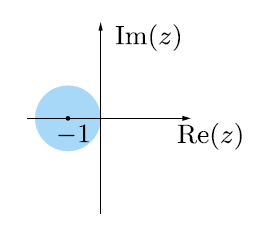
\includegraphics[width=.4\linewidth]{fig6.png}
        \label{fig:my_label}
        \end{figure}
        quindi il modo sarà \textbf{assolutamente stabile} se il suo corrispondente autovalore cadrà nella circonferenza di raggio unitario centrata in uno sul piano di Gauss
    \end{frame}
    
    \begin{frame}{Assoluta stabilità (II)}
        Per i \textbf{multistep} si analizza la regione di NON stabilità: $z= h\lambda = {\rho(e^{j\theta})\over \sigma(e^{j\theta})}$ con $\theta \in [0,2\pi]$
        $$
            \rho(\xi)=\displaystyle\sum_{j=0}^k \alpha_j\xi^{k-j}
        $$
        $$
            \sigma(\xi)=\displaystyle\sum_{j=0}^k \beta_j\xi^{k-j}
        $$
        in cui i coefficienti $\alpha_j$ e $\beta_j$ sono tratti dalla formula che descrive i metodi:
        $$
            \displaystyle\sum_{j=0}^k \alpha_jy_{n-j}=h\displaystyle\sum_{j=0}^k \beta_jf_{n-j}
        $$
    \end{frame}

    \begin{frame}{Assoluta stabilità (III)}
        \begin{figure}
        \centering
        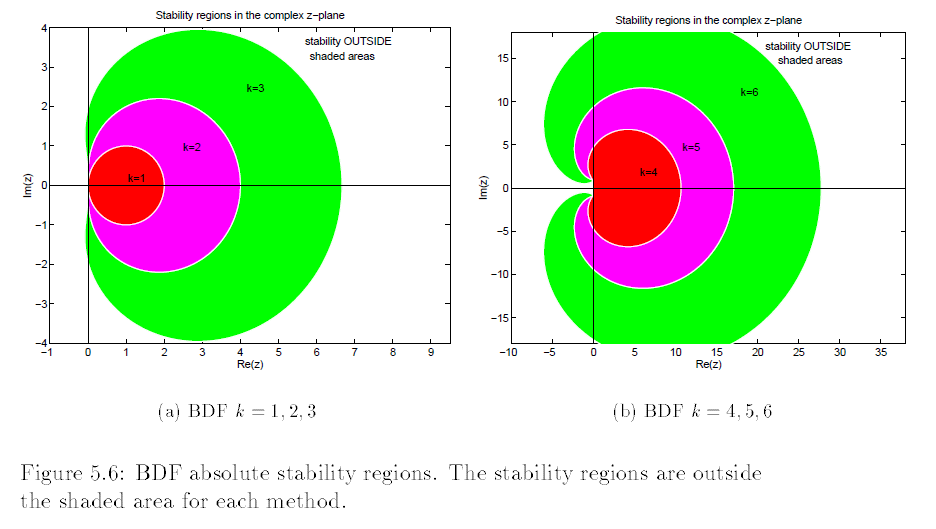
\includegraphics[width=.7\linewidth]{fig7.png}
        \label{fig:my_label}
        \end{figure}
        Vediamo che il secondo step è l’ultimo metodo che non intacca il semipiano dei reali negativi (cioè è A-stabile). 
        \begin{itemize}
            \item La risoluzione di un sistema di ODE quindi può eccitare dei modi instabili che faranno \textbf{divergere} la soluzione: l'assoluta stabilità non è sufficiente. Inoltre, oltre al sesto ordine si perde la zero-stabilità, quindi il metodo diviene inutilizzabile
        \end{itemize}
    \end{frame}



\section{Cosa sono i sistemi Stiff?}\label{sec:sec1}
\begin{frame} \frametitle{Cosa sono i sistemi Stiff?}
    \begin{itemize}
        \item Sono sistemi caratterizzati da modi (autovalori) distanti di molti ordini di grandezza tra di loro. 
        \item Più è grande la differenza tra la componente più lenta e la più veloce, più il sistema è stiff.
        \item La stiffness è una proprietà associata al sistema sotto analisi
    \end{itemize}
\end{frame}




\begin{frame}{Esempio: circuito RLC \alert{non} stiff}
Si supponga di prendere in esame il seguente circuito, con l'obiettivo di calcolarne la tensione di uscita \( V_{out}(t) \) considerando un generatore di tensione forzante \( V_{in} \)
        \begin{multicols}{2}
        \begin{center}
        \begin{circuitikz}[scale=0.8]
        \circuito 
        \end{circuitikz}
        \end{center}
    \columnbreak
    \hspace{2.5cm}
    \medskip
        \begin{cases}
            L = 67 \; m H \\
            C = 760 \; \mu F \\
            R_1 = 20 \; \Omega \\
            R_2 = 1 \; k\Omega\\
            V_{in} = V_0 \cdot \sin(2 \pi \omega t) \; V
        \end{cases} \\
        \bigskip
        \bigskip
    \hspace{2.5cm}   
    \fcolorbox{blue}{white}{
        \begin{cases}
        \lambda_1 = -100\\
        \lambda_2 = -200 \;
        \end{cases}}
    \end{multicols}
\end{frame}

\begin{frame}{Esempio: circuito RLC \alert{non} stiff - soluzione}
Il valore di \( V_{out}(t) \) è facilmente calcolato usando un metodo esplicito (eulero in avanti)

        \begin{figure}
       \centering        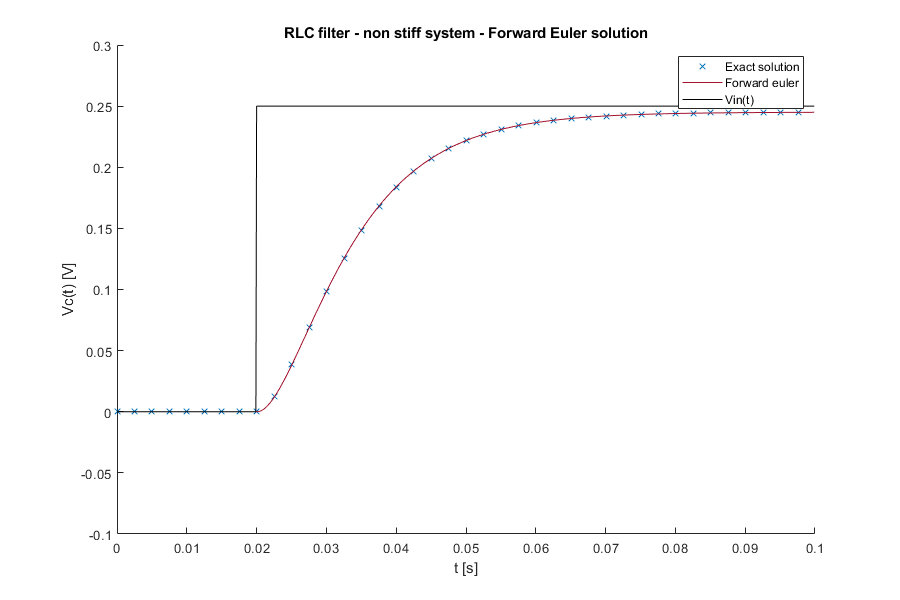
\includegraphics[width=.7\linewidth]{rlc_non_stiff_forward_euler.png}
        \label{fig:my_label}
        \end{figure}

\end{frame}

\begin{frame}{Esempio: circuito RLC stiff}
    Cambiando il valore dei componenti, il sistema dà origine ad autovalori differenti tra di loro di parecchi ordini di grandezza
        \begin{multicols}{2}
            \begin{center}
                \begin{circuitikz}[scale=0.8]
                \circuito
                \end{circuitikz}
            \end{center}
    \columnbreak
    \hspace{2.5cm}
    \medskip
        \begin{cases}
            L = 20 \; \mu H \\
            C = 500 \; \mu F \\
            R_1 = 20 \; \Omega \\
            R_2 = 1 \; k\Omega\\
            V_{in} = V_0 \cdot \sin(2 \pi \omega t) \; V
        \end{cases} \\
        \bigskip
        \bigskip
    \hspace{2.5cm}   
    \fcolorbox{red}{white}{
        \begin{cases}
            \lambda_1 = -100\\
            \lambda_2 = -1000000 \;
        \end{cases}}
    \end{multicols}
    
\end{frame}

\begin{frame}{Risolvere problemi stiff con metodi espliciti}
\begin{itemize}
    \item Per poter usare un metodo esplicito, dovremmo avere un passo dettato dall'autovalore più grande 
    \item Poiché, nel nostro esempio, l'autovalore è a frequenza altissime, il passo risulta estremamente piccolo (\( h * \lambda \ll 1 \))
\end{itemize}

        \begin{figure}
       \centering        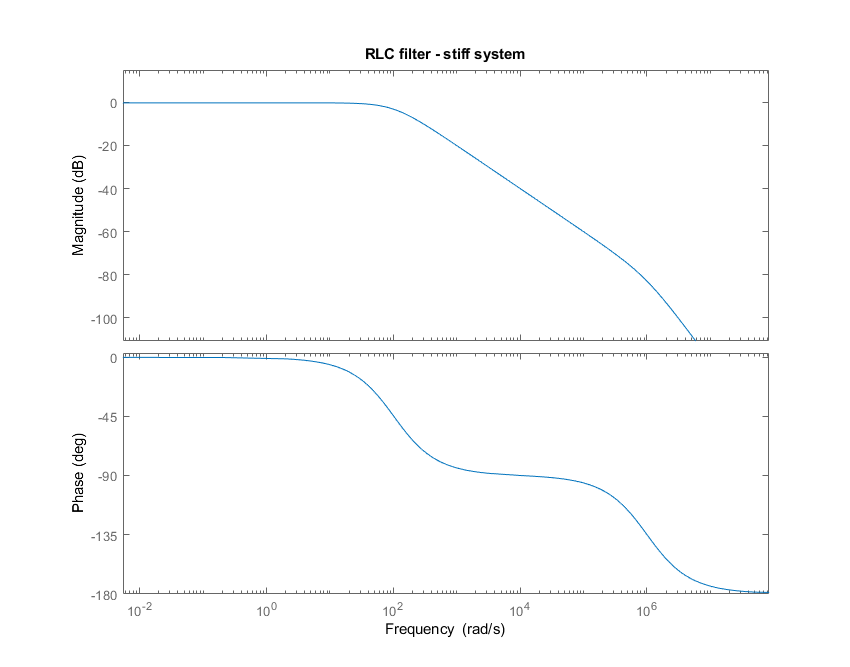
\includegraphics[width=.45\linewidth]{bode_stiff.png}
        \label{fig:my_label}
        \end{figure}
\end{frame}

\begin{frame}{Circuito RLC con eulero in avanti}
\begin{itemize}
    \item La soluzione del circuito RLC diverge se lo risolviamo con un metodo esplicito usando un passo che tiene conto solo dell'autovalore dominante
        \begin{figure}
        \centering
        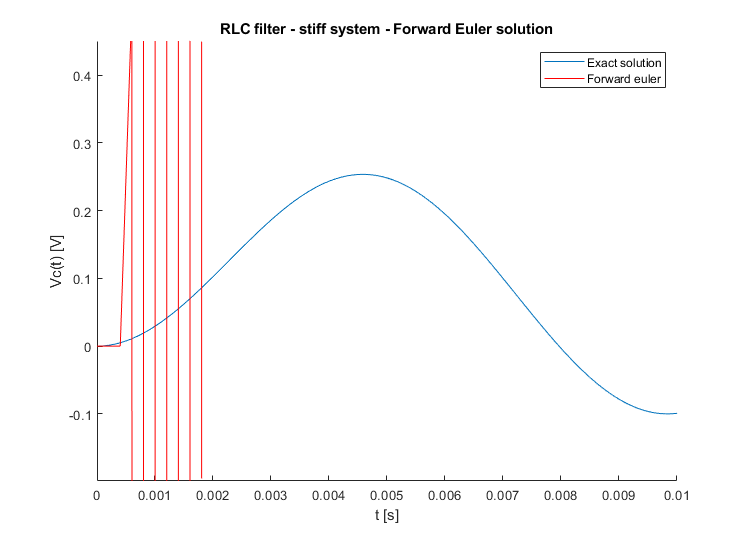
\includegraphics[width=.75\linewidth]{rlc_forward_euler.png}
        \label{fig:my_label}
        \end{figure}
\item Dovremmo inoltre fare troppi passi ($~10^{10}$) per avere il risultato della simulazione su un tempo rilevante usando una precisione che non faccia divergere il la soluzione

\item Ci servono nuovi metodi: BDF
\end{itemize}
\end{frame}

\begin{comment}
    \section{Problema risoluzione sistemi Stiff con metodi espliciti}\label{sec:sec4}

    \begin{frame}{Problema risoluzione sistemi Stiff con metodi espliciti}
        \begin{itemize}
            \item \alert{Problema modello}: con Eulero esplicito bisogna mirare al cerchio di raggio 1 (stabilità condizionata per semipiano negativo). 
            \item Per autovalori enormi, se $h\lambda$ deve centrare il cerchio, allora h (passo di discretizzazione) deve essere estremamente piccolo
            \item Per autovalori infiniti (DAE) allora  $h\approx 0$  $\rightarrow$ impossibile
            \item Possiamo risparmiare calcoli mantenendo accuratezza? Possiamo aspirare a risolvere un sistema con DAE? Bisogna ricorrere a metodi impliciti
        \end{itemize}
        
        \begin{figure}
        \centering
        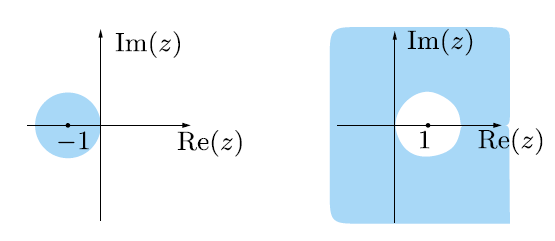
\includegraphics[width=.45\linewidth]{fig1.png}
        \caption{Per i metodi impliciti il semipiano reale negativo è tutto disponibile:\\
            \begin{itemize}
                \item h può variare incondizionatamente
                \item si possono risolvere problemi ad autovalori infiniti (DAE)
            \end{itemize}
        }
        \label{fig:my_label}
        \end{figure}
    \end{frame}
\end{comment}

\section{BDF}\label{sec:sec5}   

    \begin{frame}{BDF}
        \begin{itemize}
            \item Backward Differentiation Formulae: la valutazione n-esima dipende dalla storia passata delle valutazioni e dalla valutazione della f a passo n-esimo
            \item Sono metodi Linear Multistep (LM): 
                  sfruttano un riciclo di informazioni pregresse. \\ Ciò non Anche se lineari risolvono comunque problemi non lineari
            \[ y_n=-\displaystyle\sum_{j=1}^k \alpha_j y_{n-j} + h\beta_0 f(t_n,y_n) \]
            \[ f(y_n, t_n) = \dfrac{y_n}{h \beta_0} + \dfrac{1}{h \beta_0} \sum_{j=1}^{k}\alpha_j y_{n-j}\]
            %h\displaystyle\sum_{j=0}^k \beta_j f_{n-j} \]
        \end{itemize}
    \end{frame}
    
    \begin{frame}{BDF (II)}
        \begin{itemize}
            \item \textbf{Caso più semplice di BDF :} Eulero implicito
            \item Sono impliciti, non possiamo sfuggire dalla risoluzione di equazioni non lineari: necessitano di accoppiamento con metodi (es. Newton modificato) nell’implementazione.
        \end{itemize}
        
        %\begin{figure}
        %\centering
       % 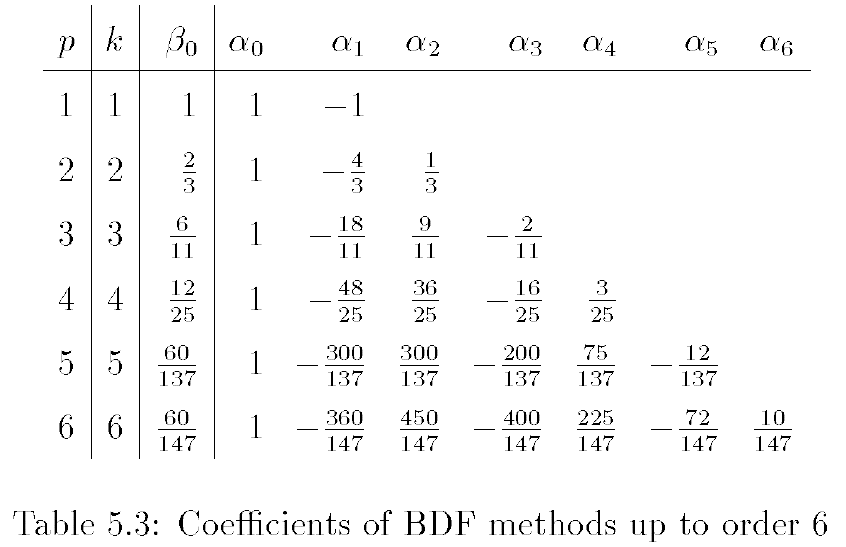
\includegraphics[width=.5\linewidth]{fig2.png}
        %\label{fig:my_label}
        %\end{figure}
        \begin{table}[]
            \begin{tabular}{Sc|Sc|Sc|ScScScScScScSc}
            \( p \) & \(k\) & \(\beta_0\) & \(\alpha_0\) & \(\alpha_1\) & \(\alpha_2\)  & \(\alpha_3\) & \(\alpha_4\) & \(\alpha_5\) & \(\alpha_6\) \\
            \hline
            \(1\) & \(1\) & \(1 \)       & \(1 \) & \(-1\)       &                             &          &         &         &        \\
            \(2\) & \(2\) & \(\sfrac{2}{3} \)    & \(1\) & \(\sfrac{4}{3} \)     & \(\sfrac{1}{3} \)                         &          &         &         &        \\
            \(3\) & \(3\) & \(\sfrac{6}{11} \)   & \(1\) & \(\sfrac{-18}{11} \)   & \(\sfrac{9}{1} \)                       & \(\sfrac{-2}{11}\)    &         &         &        \\
            \(4\) & \(4\) & \(\sfrac{12}{25} \)  & \(1\) & \(\sfrac{-48}{25} \)   & \(\sfrac{36}{25} \)   & \(\sfrac{-16}{25}\)   & \(\sfrac{3}{25}\)   &         &        \\
            \(5\) & \(5\) & \(\sfrac{60}{137} \) & \(1\) & \(\sfrac{300}{137} \)  & \(\sfrac{300}{137}\) & \(\sfrac{-200}{137}\) & \(\sfrac{75}{137}\)  & \(\sfrac{-12}{137}\) &        \\
            \(6\) & \(6\) & \(\sfrac{60}{147} \) & \(1\) & \(\sfrac{-360}{147} \) & \(\sfrac{450}{147}\) & \(\sfrac{-400}{137}\) & \(\sfrac{225}{147}\) & \(\sfrac{72}{147}\) & \(\sfrac{10}{147}\)
            \end{tabular}
        \end{table}
        

        
        
    \end{frame}

\begin{frame}{BDF (IV)}
        \begin{itemize}
            \item {La tabella può essere meglio visualizzata scrivendo le equazioni $\alpha_j$ e $\beta_0$:}
        \end{itemize}
        
    \begin{center}
        \begin{table}[]
            \begin{tabular}{ScSl}
            BDF1 & \( y_{n+1} = y_n + h f(t_{n+1}, y_{n+1})\) \textcolor{red}{\rightarrow \( y_{n+1} = -\alpha_1y_n + \beta_0h f(t_{n+1}, y_{n+1})\)}\\
            BDF2 & \(y_{n+2} = \tfrac43 y_{n+1} - \tfrac13 y_n + \tfrac23 h f(t_{n+2}, y_{n+2}) \) \textcolor{red}{\rightarrow \(y_{n+2} = -\alpha_1y_{n+1} -\alpha_2y_n + \beta_0h f(t_{n+2}, y_{n+2}) \)}\\
            
            BDF3 & ...\\%\(y_{n+3} = \tfrac{18}{11} y_{n+2} - \tfrac9{11} y_{n+1} + \tfrac2{11} y_n +\tfrac6{11} h f(t_{n+3}, y_{n+3}) \) \\
            BDF4 & ...\\ %\(y_{n+4} = \tfrac{48}{25} y_{n+3} - \tfrac{36}{25} y_{n+2} + \tfrac{16}{25} y_{n+1} - \tfrac{3}{25} y_n + \tfrac{12}{25} h f(t_{n+4}, y_{n+4}) \) \\
            BDF5 & ...\\ %\( y_{n+5} = \tfrac{300}{137} y_{n+4} - \tfrac{300}{137} y_{n+3} + \tfrac{200}{137} y_{n+2} - \tfrac{75}{137} y_{n+1} + \tfrac{12}{137} y_n + \tfrac{60}{137} h f(t_{n+5}, y_{n+5}) \)  \\
            BDF6 & \(y_{n+6} + \tfrac{360}{147} y_{n+5} - \tfrac{450}{147} y_{n+4} + \tfrac{400}{147} y_{n+3} - \tfrac{225}{147} y_{n+2} + \tfrac{72}{147} y_{n+1} - \tfrac{10}{147} y_n + \tfrac{60}{147} h f(t_{n+6}, y_{n+6}) \) 
            \end{tabular}
        \end{table}
    \end{center}
\end{frame}

\section{Vantaggi e svantaggi}\label{sec:sec6} 

    \begin{frame}{Vantaggi e svantaggi}
        \textbf{Vantaggi:}
        \begin{itemize}
            %\item Richiedono meno valutazioni della funzione per ogni step (rispetto a Runge-Kutta)
            \item Migliore accuratezza rispetto ad altri metodi (es. RK) a parità di numero di valutazioni della funzione
            \item Metodi costruiti più semplici e performanti in fatto di ordine e stima dell’errore 
            %\item Migliore accuratezza rispetto a metodi one-step a parità di numero di valutazioni della funzione
        \end{itemize}
        \textbf{Svantaggi:}
        \begin{itemize}
            \item Necessità di condizioni iniziali accurate: alto costo computazionale di partenza 
            \item Flessibilità minore per avere adattività di ordine e di passo di integrazione
            \item Per metodi multistep: zero stabilità da determinare (gli one step hanno la zero stabilità garantita dalla consistenza)
        \end{itemize}
    \end{frame}

\section{Priming}\label{sec:sec7}
    \begin{frame}{Problema del priming: ricerca dei valori iniziali}
        \begin{itemize}
            \item Stabilire i valori iniziali di una risoluzione per BDF non è banale.
            \item Se i valori non sono di accuratezza adeguata $O(h^p)$, il metodo non converge a ordine massimo.
            \item Esempio: metodo-5 step. Non è possibile partire subito, mancano gli step precedenti.\\ 
            È d'obbligo fornire (calcolare) i valori precedenti con altri metodi.
            \item Metodi usati per i valori iniziali: RK, uso ricorsivo di metodi a passi precedenti
        \end{itemize}   
    \end{frame}
    
\section{Ordine e consistenza}\label{sec:sec8}
    \begin{frame}{Ordine e consistenza }
        \begin{itemize}
            \item Per i metodi LM questa operazione risulta particolarmente semplice.
        \end{itemize}
        \begin{itemize}
            \item Come visto a lezione per il caso Eulero all'indietro, analizziamo l'errore di troncamento e vediamo se è trascurabile rispetto a $h^p$.
            \item Lo stesso ragionamento viene applicato ai metodi multistep tramite opportuno operatore lineare. 
            \item Lo sviluppo di Taylor ricavato per più step sarà: 
        \end{itemize}
        
          \[L_{h}y(t) = C_0y(t) + C_1hy'(t) + ... + C_qh^qy^{(q)}(t) + ...   \textnormal{ in cui }\]
          \[ C_0 = \displaystyle\sum_{j=0}^k \alpha_j \textnormal{ e }  C_i = (-1)^i \biggl[{1 \over i!}\displaystyle\sum_{j=1}^k j^i\alpha_j  + {1 \over (i - 1)!} \displaystyle\sum_{j=0}^k j^{i-1}\beta_j\biggl] \textnormal{ con } i = 1, 2, 3, ...\]
          \[ \textnormal{ L'errore di troncamento locale è } d_n = {L_h[y(t_n)] \over h} \textnormal{ in cui  } y(t_n) \textnormal{ è la soluzione esatta al punto } t = t_n .\]
    \end{frame}

\begin{frame}{Ordine e consistenza (II)}
        \begin{itemize}
            \item Si dice che il metodo ha ordine $p$ se l'errore di troncamento locale è $d_n = O(h^p)$.
        \end{itemize}
        \begin{itemize}
            \item E' possibile tradurre questa informazione in $C_i$, diremo che il metodo è di ordine $p$ se:
        \end{itemize}
        \[ C_0 = C_1 = ... = C_p = 0 \textnormal{ con } C_{p+1} \not= 0 \]
         \begin{itemize}
            \item E' possibile inoltre dimostrare che il metodo è consistente se e solo se:
        \end{itemize}
        \centering$ \displaystyle\sum_{j=0}^k \alpha_j = 0  $ \space\space\space  e\space\space \space  $  \displaystyle\sum_{j=1}^k j\alpha_j + \displaystyle\sum_{j=0}^k \beta_j = 0$
        \begin{itemize}
            \item Scrivendo i polinomi caratteristici del metodo:\\
            \centering$ \rho(\xi) = \displaystyle\sum_{j=0}^k \alpha_j\xi^{k-j}$  \space\space\space \sigma(\xi) = \displaystyle\sum_{j=0}^k \beta_j\xi^{k-j} $\\
            \flushleft la condizione di consistenza diventa (se e solo se) per $\rho(1) = 0$ e $\rho'(1) = \sigma(1)$.
        \end{itemize}
   \end{frame}
\section{Zero stabilità e convergenza}\label{sec:sec9}
    \begin{frame}{Zero stabilità e convergenza}
        \begin{itemize}
            \item La zero stabilità per BDF (ed in generale metodi LM) deve essere analizzata per ogni ordine del metodo.
        \end{itemize}   
        Proviamo a dare qualche definizione.
        \begin{itemize}
            \item Si dice \alert{zero stabile} se è in grado di risolvere correttamente \( y'=0 \), cioè per una perturbazione del calcolo all’interno del metodo, la soluzione non diverge
        \end{itemize}
        
       Facciamo un semplice esempio:
        \[u_{n+1} = 5 u_n + u_{n-1}  \textnormal{ con } f = 0\]
        \begin{center}
         \begin{pmatrix}
            u_{n+1} \\ 
            u_{n}
         \end{pmatrix}
         =
         \begin{bmatrix}
                    5 & 1 \\
                    1 & 0
         \end{bmatrix}
        \begin{pmatrix}
            u_{n} \\ 
            u_{n-1}
         \end{pmatrix}
         \end{center}
         \[\vec{u_n} = A \vec{u_{n-1}} = AA \vec{u_{n-2}}= A^{n+1} \vec{u_0} \]
         \[A = U \Lambda U ^ {-1} \textnormal{ con } \Lambda \textnormal{ matrice contenente gli autovalori} \]
         \[AA = (U \Lambda U^{-1})(U \Lambda U^{-1}) = U \Lambda (U^{-1} U) \Lambda U^{-1} = U \Lambda \Lambda U^{-1} \]
         \[A^{n+1} = U \Lambda^{n+1} U^{-1}\]
       % \begin{figure}
       % \centering
       % 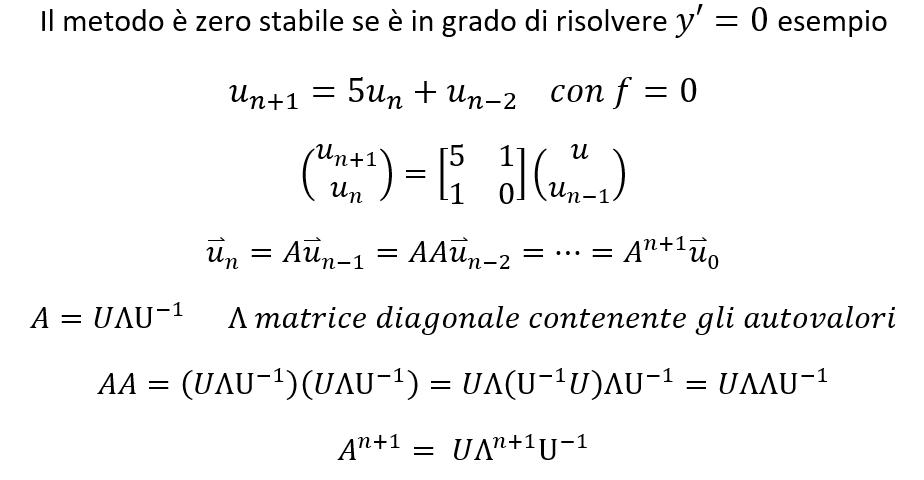
\includegraphics[width=.5\linewidth]{fig3.png}\\
       % 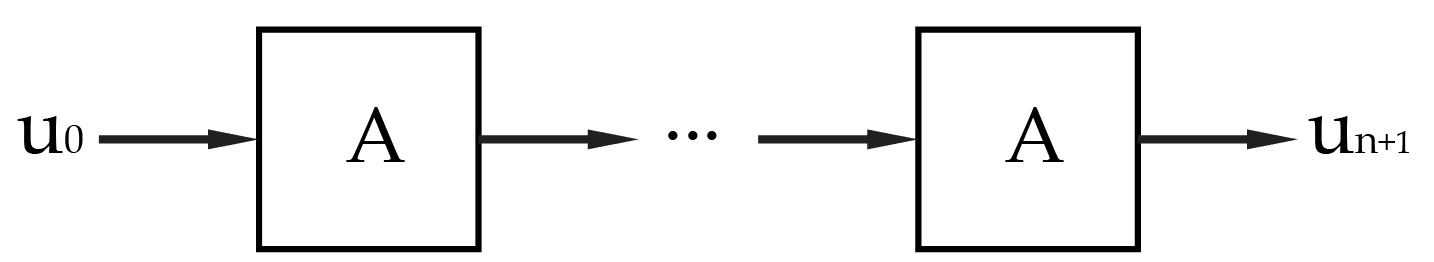
\includegraphics[width=.4\linewidth]{fig4.png}
        %\label{fig:my_label}
       % \end{figure}
       
       \begin{center}




\tikzset{every picture/.style={line width=0.75pt}} %set default line width to 0.75pt        

\begin{tikzpicture}[x=0.75pt,y=0.75pt,yscale=-1,xscale=1]
%uncomment if require: \path (0,377); %set diagram left start at 0, and has height of 377

%Straight Lines [id:da6413889010993787] 
\draw    (219.75,42.5) -- (242.75,42.5) ;
\draw [shift={(244.75,42.5)}, rotate = 180] [color={rgb, 255:red, 0; green, 0; blue, 0 }  ][line width=0.75]    (10.93,-3.29) .. controls (6.95,-1.4) and (3.31,-0.3) .. (0,0) .. controls (3.31,0.3) and (6.95,1.4) .. (10.93,3.29)   ;
%Shape: Rectangle [id:dp2986809547616538] 
\draw   (249.75,27.5) -- (279.75,27.5) -- (279.75,57.5) -- (249.75,57.5) -- cycle ;
%Straight Lines [id:da425759494133338] 
\draw    (284.75,42.5) -- (307.75,42.5) ;
\draw [shift={(309.75,42.5)}, rotate = 180] [color={rgb, 255:red, 0; green, 0; blue, 0 }  ][line width=0.75]    (10.93,-3.29) .. controls (6.95,-1.4) and (3.31,-0.3) .. (0,0) .. controls (3.31,0.3) and (6.95,1.4) .. (10.93,3.29)   ;
%Straight Lines [id:da27927127529816453] 
\draw    (336.25,42.5) -- (359.25,42.5) ;
\draw [shift={(361.25,42.5)}, rotate = 180] [color={rgb, 255:red, 0; green, 0; blue, 0 }  ][line width=0.75]    (10.93,-3.29) .. controls (6.95,-1.4) and (3.31,-0.3) .. (0,0) .. controls (3.31,0.3) and (6.95,1.4) .. (10.93,3.29)   ;
%Straight Lines [id:da4618389576336408] 
\draw    (401.25,42.5) -- (424.25,42.5) ;
\draw [shift={(426.25,42.5)}, rotate = 180] [color={rgb, 255:red, 0; green, 0; blue, 0 }  ][line width=0.75]    (10.93,-3.29) .. controls (6.95,-1.4) and (3.31,-0.3) .. (0,0) .. controls (3.31,0.3) and (6.95,1.4) .. (10.93,3.29)   ;
%Shape: Rectangle [id:dp45653346798672434] 
\draw   (370,30) -- (400,30) -- (400,60) -- (370,60) -- cycle ;

% Text Node
\draw (198,39) node [anchor=north west][inner sep=0.75pt]  [font=\normalsize] [align=left] {$\displaystyle u_{0}$};
% Text Node
\draw (259.4,37) node [anchor=north west][inner sep=0.75pt]  [font=\normalsize] [align=left] {$\displaystyle A$};
% Text Node
\draw (316,43) node [anchor=north west][inner sep=0.75pt]  [font=\normalsize] [align=left] {$\displaystyle ...$};
% Text Node
\draw (429,37) node [anchor=north west][inner sep=0.75pt]  [font=\normalsize] [align=left] {$\displaystyle u_{n+1}$};
% Text Node
\draw (380.6,38.6) node [anchor=north west][inner sep=0.75pt]  [font=\normalsize] [align=left] {$\displaystyle A$};


\end{tikzpicture}

       \end{center}

\end{frame}
    
    \begin{frame}{Zero stabilità e convergenza (II)}
        \begin{itemize}
            \item Se gli autovalori hanno modulo $>1$, al passo n-esimo la matrice $A^{n+1}$ avrà coefficienti enormi. Nel nostro caso, gli autovalori sono  $0.19258$ e $5.19258$
            \item Al ventesimo passo, la $A^{n+1}$ sarà: 
            %\[ 1.0e\+14 \]
            \vspace{0.5cm}
            \begin{center}
                \begin{bmatrix} 
                1.958*10^{14} & 0.377*10^{14} \\ 
                0.377*10^{14} & 0.0726*10^{14}
                \end{bmatrix} 
            \end{center}
            \vspace{0.5cm}
            
            %\begin{figure}
           % \flushleft
            %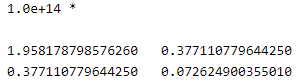
\includegraphics[width=.4\linewidth]{fig5.png}
            %\label{fig:my_label}
            %\end{figure}
            
            Qualsiasi perturbazione introdotta nel metodo verrà amplificata, anche solo un semplice errore nel valore iniziale.
            \medskip
            \medskip
            \item La BDF del secondo ordine zero stabile ha autovalori 1 e $1/3$
        \end{itemize} 
    \end{frame}
    
    \begin{frame}{Zero stabilità e convergenza (III)}
        Concludendo: il metodo è \textbf{zero stabile} se tutte le radici $\xi_i$ (gli autovalori associati al metodo) del polinomio caratteristico $\rho(\xi)$ soddisfano $|\xi_i|\leq1$, in cui 
        $$
            \rho(\xi)=\displaystyle\sum_{j=0}^k \alpha_j\xi^{k-j}
        $$
    \end{frame}


    
\section{Stiff decay}\label{sec:sec11}    
    \begin{frame}{Stiff Decay}
        È una proprietà associata al metodo di risoluzione.
        Non è una buona idea accontentarsi dell’A-stabilità (stabilità nel semipiano dei reali negativi) quando si parla specialmente di sistemi stiff. 
        Infatti, ci sono due casi in cui non è una condizione sufficientemente stringente:
        \begin{itemize}
            \item $\Re(\lambda)<<1$ (autovalori a velocità molto alta)
            \item $1<<\Re(\lambda)\leq0$ e $|\Im(\lambda)|>>1$ (grandi oscillazioni per valori complessi vicini all’asse immaginario
        \end{itemize}
        Considerando l’equazione di test $y'= \lambda(y-g(t))$, riscrivibile come $\epsilon y'= \epsilon\lambda(y-g(t))$ dove $\epsilon=\frac{1}{Re(\lambda)}$, si noti che per $\epsilon=0$ si ottiene la soluzione $y(t) = g(t)$. \\
        Questo si motiva dicendo che il metodo di discretizzazione ha \textit{stiff decay} se fissato $t_n>0$, $|y_n-g(t_n)|\rightarrow 0$ per $h_n\Re(\lambda)\rightarrow -\infty$.\\
        Analizzando il metodo di \textbf{Eulero all’indietro} si conclude che esso ha stiff decay, infatti applicando l’equazione $\epsilon y'= \epsilon\lambda(y-g(t))$ si ottiene: $$y_n-g(t_n)=(1-h_n-\lambda)^-^1(y_n_-_1-g(t_n))$$
        
    \end{frame}
    
    \begin{frame}{Stiff Decay (II)}
        Questo non vale per il metodo di Eulero in avanti che non ha stiff decay.\\
        \medskip
        \medskip
        Si può dire che lo stiff decay è quindi un \alert{indice} che rivela quanto un metodo di risoluzione sia veloce nell’assestarsi alla soluzione di un sistema stiff.
        Difatti, il vantaggio nell'uso dei metodi con \textit{stiff decay} è la loro capacità di \textbf{trascurare la parte della soluzione che varia velocemente} senza però perdere dettagli nella parte a bassa velocità.
        \begin{figure}
        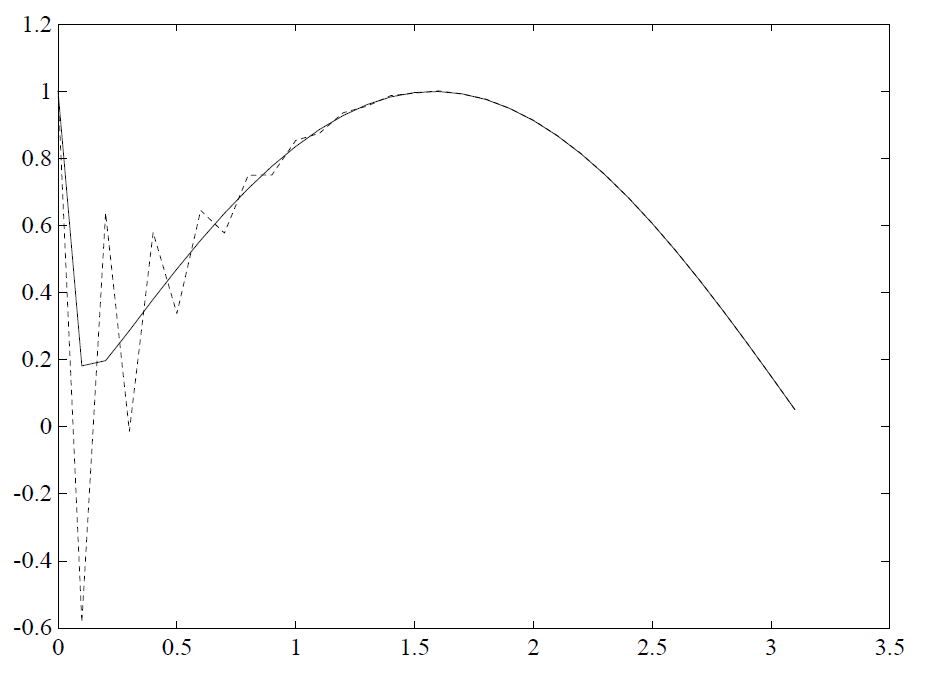
\includegraphics[width=.4\linewidth]{fig8.png}
        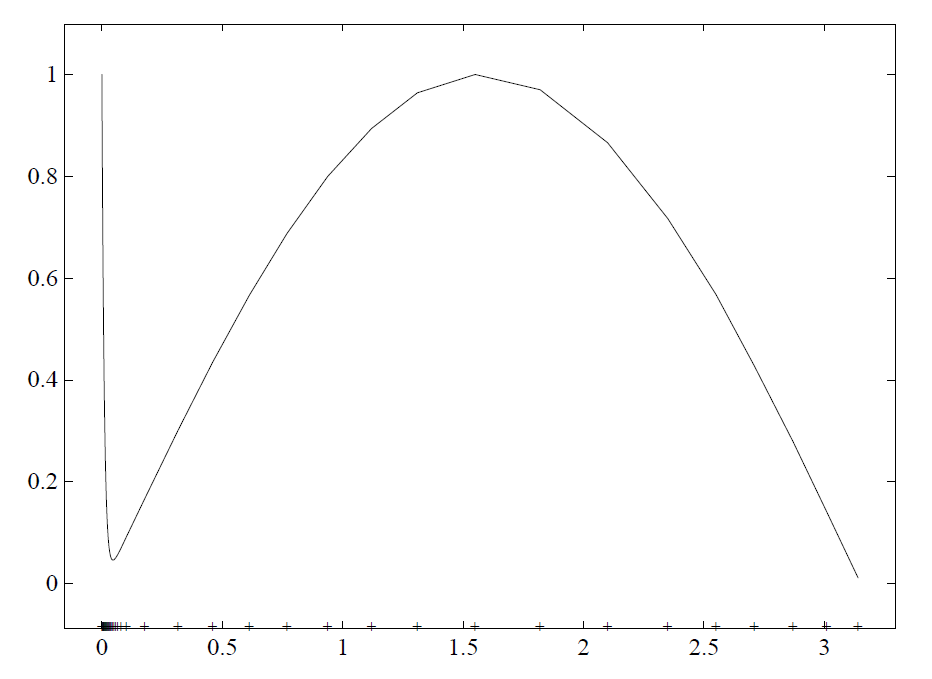
\includegraphics[width=.4\linewidth]{fig9.png}
        \label{fig:my_label}
    \end{figure}
        
    \end{frame}

\section{Implementazione}\label{sec:sec12}  
\begin{frame}{Priming}
come risolviamo il priming in matlab
 \end{frame}
\begin{frame}{Risoluzione di eq non lineari con fsolve}
tbd
 \end{frame}
 \begin{frame}{Circuito RLC - soluzioni con BDF}
    \begin{figure}
        \centering
        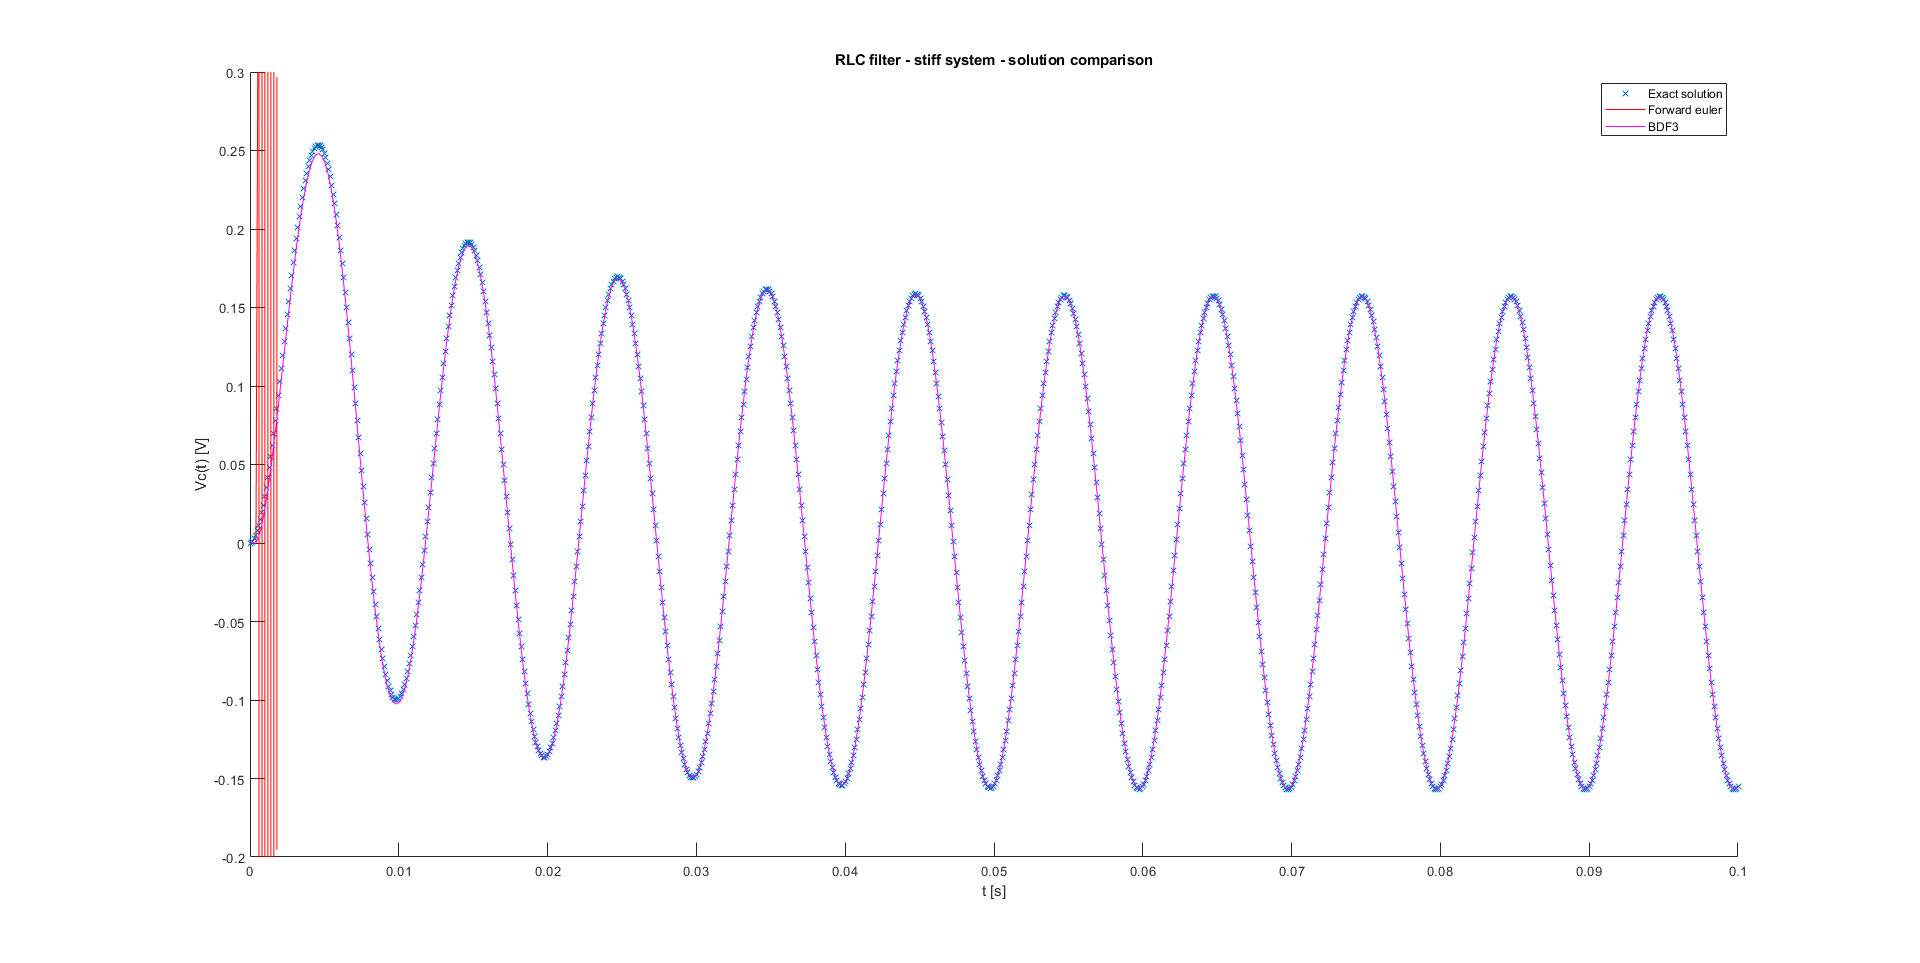
\includegraphics[width=.9\linewidth]{rlc_solution_comparison.png}
        \label{fig:my_label}
    \end{figure}
 \end{frame}
\begin{frame}{Circuito RLC - al variare del passo?}
scegliere un metodo bdf e risolvere il circuito con diversi passi, plottando l'errore in funzione di h
 \end{frame}
\begin{frame}{Reazione chimica}
soluzioni della reazione - concentrazione dei reagenti nel tempo ( $~10^{11}$ )  
 \end{frame}
\end{document}
